\documentclass{beamer}
\usepackage{graphics}
\usepackage{epsfig}
\usepackage{multicol}
\usepackage{pifont}
\setbeamertemplate{navigation symbols}{}
\newcommand{\RR}{\ensuremath{\mathbb{R}}}
\newcommand{\NN}{\ensuremath{\mathbb{N}}}
\newcommand{\QQ}{\ensuremath{\mathbb{Q}}}
\newcommand{\CC}{\ensuremath{\mathbb{C}}}
\newcommand{\ZZ}{\ensuremath{\mathbb{Z}}}
\newcommand{\TT}{\ensuremath{\mathbb{T}}}
\newcommand{\HH}{\ensuremath{\mathbb{H}}}
\DeclareMathOperator{\Min}{Min}
\DeclareMathOperator{\mint}{min}
\DeclareMathOperator{\vertt}{vert}
\DeclareMathOperator{\conv}{conv}
\DeclareMathOperator{\rank}{rank}

\def\QuotS#1#2{\leavevmode\kern-.0em\raise.2ex\hbox{$#1$}\kern-.1em/\kern-.1em\lower.25ex\hbox{$#2$}}

\begin{document}
\title{Implicit schemes for wave models}
\author{
\begin{center}
\textcolor{red}{\large Mathieu Dutour Sikiri\'c}\\[2mm]
\textcolor{red}{Rudjer Bo\u skovi\'c Institute, Croatia}\\[2mm]
\textcolor{red}{and Universit\"at Rostock}
\end{center}
}

\date{\today} 
\frame{\titlepage} 








\frame{
\begin{center}
\begin{tabular*}{7cm}{c}
\\[-0.5cm]
{\Huge \textcolor{blue}{I. }\textcolor{red}{Wave models}}
\end{tabular*}
\end{center}
}

\frame{
  \frametitle{Stochastic wave modelling}

\begin{itemize}
\item Oceanic models are using grids (structured or unstructured) of size $1km\leq d\leq 10km$ to simulate the ocean
\item But oceanic waves have a typical wavelength $2m$ $\leq$ $L$ $\leq$ $100m$. So, we cannot resolve waves in the ocean.
\item But if one uses phase averaged models and uses stochastic assumptions
then it is possible to model waves by a spectral wave action density
$N({\bf x},{\bf k})$
\item This density satisfies a Wave Action Equation (\textcolor{red}{WAE}) which represents advection, refraction, frequency shifting and source terms:
\begin{equation*}
\frac{\partial N}{\partial t} + \nabla_x(({\bf c}_g+{\bf u}_A)N) + \nabla_k(\dot{k} N) 
 + \nabla_{\theta}(\dot{\theta} N) = S_{tot}
\end{equation*}
with
\begin{equation*}
S_{tot} = S_{in} + S_{nl3} + S_{nl4} + S_{bot} + S_{ds} + S_{break} + S_{bf}
\end{equation*}
\end{itemize}
}

\frame{
  \frametitle{The WWM model}
\begin{itemize}
\item The Wind Wave Model (WWM) is a unstructured grid spectral wave model.
\item It is comparable to WaveWatch III, SWAN, WAM or SWAVE.
\item It incorporates most existing source term formulation for wind input and dissipation (Cycle III, Cycle IV, Ardhuin, Makin, ...)
\item It has been coupled to SELFE, SHYFEM, TIMOR and ROMS.
\item It uses Residual Distribution schemes for the horizontal advection.
\item It integrates the WAE by using the Operator Splitting Method in explicit or implicit mode.
\end{itemize}
}



\frame{
  \frametitle{Operator Splitting Method}
\begin{itemize}
\item A standard technique for integrating partial differential equations is the operator splitting method.
\item Over the interval $[t_0, t_1]$ we successively solve the equations
\begin{equation*}
\left\lbrace\begin{array}{rcl}
\frac{\partial N_1}{\partial t} + \nabla_{\theta}(\dot{\theta} N_1) = 0  &\mbox{~with~}& N_1(t_0)=N(t_0)\\ 
\frac{\partial N_2}{\partial t} + \nabla_k(\dot{k} N_2) = 0  &\mbox{~with~}& N_2(t_0)=N_1(t_1)\\ 
\frac{\partial N_3}{\partial t} + \nabla_x(({\bf c}_g+{\bf u}_A)N_3) = 0 &\mbox{~with~}& N_3(t_0) = N_2(t_1)\\
\frac{\partial N_4}{\partial t} = S(t) &\mbox{~with~}& N_4(t_0) = N_3(t_1)\\
\end{array}\right.
\end{equation*}
and we set $N(t_1)=N_4(t_1)$.
\item No matter what the order of the successive integration schemes is the final order will be $1$.
\item It it is possible to have higher order by more complex integration procedures (Strang splitting, iterative splitting, etc.)
\end{itemize}
}

\frame{
  \frametitle{The CFL criterion}
\begin{itemize}
\item If the discretization has characteristic length $l$ and the physical speed is $c$ then we have the condition
\begin{equation*}
\frac{ c \Delta t}{l} \leq 1
\end{equation*}
\item For the integration of the frequency and directional equations we can subdivide the integration time step if necessary because everything is decoupled.
\item This is not possible for the geographical advection:
\begin{itemize}
\item The dependency in direction/frequency is small or negligible
\item The problem is that the group speed is $\sqrt{g h}$ and so the CFL number varies with the depth and the resolution.
\end{itemize}
\item So, we will present an implicit scheme for integrating $N_1$, i.e. in order to avoid the CFL limitation for advection.
\item Remark: the advection scheme used in implicit mode in WWM is the residual distribution scheme PSI.
\end{itemize}
}




\frame{
\begin{center}
\begin{tabular*}{7cm}{c}
\\[-0.5cm]
{\Huge \textcolor{blue}{II. }\textcolor{red}{MPI}}\\[4mm]
{\Huge \textcolor{red}{parallelization}}
\end{tabular*}
\end{center}
}







\begin{frame}[fragile]
  \frametitle{{\tt MPI} parallelization I}
\begin{itemize}
\item The parallelization of geophysical models is usually done by using the Mesage Passing Interface {\tt MPI} formalism.
\item The set of computational nodes of the model is thus split into a number of different subdomains.
\item in {\tt MPI} the exchanges are explicit. The explicit way of doing it is via:
\begin{verbatim}
CALL MPI_SEND(ArrSend,len,dest,tag,comm,ierr)
CALL MPI_RECV(ArrRecv,len,orig,tag,comm,istat,ierr)
\end{verbatim}
Those operations are blocking, i.e. the program waits until all sends and recvs have been processed.
\item This means that all exchanges are processed by the order in which they are stated.
\item It is generally better to decrease the total number of exchanges in order to get better performance.
\end{itemize}
\end{frame}


\begin{frame}[fragile]
  \frametitle{{\tt MPI} parallelization II}
\begin{itemize}
\item In order to avoid strictly ordained exchanges, the strategy is to do asynchrone exchanges.
\item The procedure is done in the following way
\begin{verbatim}
DO iorig=1,nproc
  CALL MPI_IRECV(U,1,type(iorig), iorig-1, tag, 
       comm, rqst(iorig), ierr)
END DO
CALL MPI_WAITALL(nproc,rqst, stat, ierr)
\end{verbatim}
and similarly for send operations.
\item The idea is the following: the array {\tt type(iorig)} contains the list of positions at which the received data needs to be put. Commands for creating such types are for example {\tt mpi\_create\_indexed\_block}.
\item By using the above the order of the exchanges is no longer determined by the MPI program which makes it faster but harder to debug.
\end{itemize}
\end{frame}


\frame{
\begin{center}
\begin{tabular*}{7cm}{c}
\\[-0.5cm]
{\Huge \textcolor{blue}{II. }\textcolor{red}{Iterative solution}}\\[4mm]
{\Huge \textcolor{red}{methods}}
\end{tabular*}
\end{center}
}






\frame{
  \frametitle{Iterative solution methods}
\begin{itemize}
\item In order to resolve linear system $Ax = b$ for typical geophysical situation we have matrices of size $N\times N$ with $N$ about $100000$
\item We cannot use direct methods like Gauss elimination or $LU$ and so we need to use iterative methods.
\item For a matrix $A$ and a vector $b$ the Krylov space $K_n(A,b)$ is
\begin{equation*}
K_n(A,b)=Vect \left\{ b, Ab, \dots, A^{n-1}b \right\}
\end{equation*}
\item The Generalized Minimal Residual Method (GMRES) takes the best solution in $K_n(A,b)$ of $Ax = b$.
\item It is stable but it requires the storing of $n$ vectors, which is memory intensive.
\item So, in order to have a good solution strategy we need a method with minimal storage requirement.
\end{itemize}
}

\frame{
  \frametitle{The conjugate gradient method}
\begin{itemize}
\item If the matrix $A$ is positive definite, then the conjugate gradient method can be used:
\begin{itemize}
\item[\textcolor{red}{\ding{224}}] 
J.W. Shewchuk, {\em An Introduction to the Conjugate Gradient Method Without the Agonizing Pain} Edition 1$\frac{1}{4}$
\end{itemize}
\begin{itemize}
\item If the system is $N$ dimensional then $N$ iteration suffices.
\item After $i$ iterations, the residual error $e_i$ satisfies
\begin{equation*}
\left\Vert e_i \right\Vert \leq 2 \left(\frac{\sqrt{\kappa} - 1}{\sqrt{\kappa} + 1}\right)^i \left\Vert e \right\Vert_0 \mbox{~with~}\kappa = \frac{\lambda_{max}}{\lambda_{min}}
\end{equation*}
\item Operations depends on computing $Ax$ for some vectors $x$.
\end{itemize}
\item For non-symmetric problems, the technique is to use the biconjugate gradient stabilized (BCGS) which works similarly.
\end{itemize}
}


\frame{
  \frametitle{Preconditioners}
\begin{itemize}
\item The convergence of the conjugate gradient depends on $\kappa$ that is on how far $A$ is from the identity matrix.
\item If $\kappa$ is large, i.e. $A$ is ill conditioned then the number of iterations will be very large.
\item We may accept that but then the whole solution strategy becomes very similar to an explicit scheme.
\item The idea is to find a matrix $K$ for which we can compute the inverse easily.
\item $K$ must similar to $A$, i.e. share the same property as $A$.
\item In order to apply the BCGS we need to compute $Ax$ and $K^{-1}x$ for some vectors $x$.
\item Example: Jacobi preconditioning is to take the diagonal entries of $A$.
\end{itemize}
}


\frame{
  \frametitle{Preconditioners for advection}
\begin{itemize}
\item The essential aspect of advection is that it moves things so Jacobi preconditioner will not work.
\item Instead partial factorization techniques have to be used
\item We write $A = D + E + F$ with $D$ diagonal $E$ lower triangular and $F$ upper triangular.
\item The Successive Over Relaxation (SOR) preconditioner is to say
\begin{equation*}
A = (I + ED^{-1})(D + F) + R \mbox{~with~} R= -E D^{-1} F
\end{equation*}
\item The incomplete LU factorization (ILU0) is to say
\begin{equation*}
A_{ij} = (LU)_{ij} \mbox{~for~} A_{ij}\not= 0
\end{equation*}
with $L$ and $U$ having the same sparsity as $A$.
\item Both methods are efficient because they both are of the form $K = LU$.
\item So, when solving $Kx = b$ we do
\begin{equation*}
x' = L^{-1} b \mbox{~and~} x=U^{-1} x',
\end{equation*}
i.e. the solution propagates.
\end{itemize}
}




\frame{
\begin{center}
\begin{tabular*}{7cm}{c}
\\[-0.5cm]
{\Huge \textcolor{blue}{II. }\textcolor{red}{Parallelizing}}\\[4mm]
{\Huge \textcolor{red}{solvers}}
\end{tabular*}
\end{center}
}





\frame{
  \frametitle{Parallelizing solvers}
\begin{itemize}
\item Suppose we have to solve $Lx = b$ and let us assume the diagonal is $1$.
\begin{equation*}
\left\{\begin{array}{lcl}
x_1                             &=& b_1\\
l_{2,1} x_1 + x_2                 &=& b_2\\
\vdots                         &\vdots &\vdots\\
l_{N, 1} x_1 + \dots + l_{N,N-1} x_{N-1} + x_N &=& b_N
\end{array}\right.
\end{equation*}
So, we first determine $x_1$ then $x_2$ and finally $x_N$.
\item Parallelization is impossible if all $L_{ij}$ are non-zeros because data from one processor
\item What save us is sparsity because the matrices are of the following type:
\begin{equation*}
f(x)_v = \sum_{v' \sim v} C_{v,v'} x_{v'}
\end{equation*}
with $v \sim v'$ mean that $v$ and $v'$ are adjacent nodes.
\end{itemize}
}

\frame{
  \frametitle{Ordering nodes}
\begin{itemize}
\item All incomplete factorizations depend on the ordering of the nodes.
\item We are free to choose the ordering that suits us best and by doing so we change the preconditioner $LU$.
\item Since the iterative solution algorithms return approximate solutions this means that the approximate solutions depend on the partitioning and also on the number of processors.
\item The situation is the following:
\begin{center}
\begin{minipage}[b]{5.2cm}
\centering
\resizebox{4.0cm}{!}{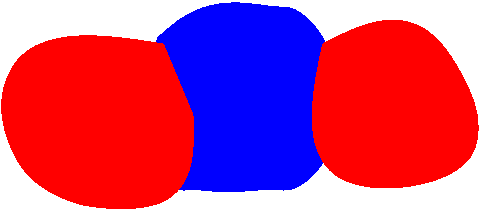
\includegraphics{ImplPic/ColorDomain.pdf}}\par
Colored domains
\end{minipage}
\begin{minipage}[b]{3.2cm}
\centering
\resizebox{2.5cm}{!}{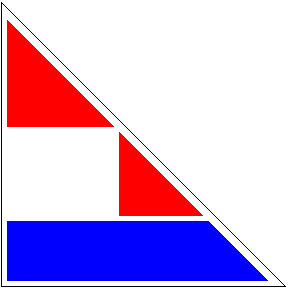
\includegraphics{ImplPic/Lmatrix.pdf}}\par
The $L$ matrix
\end{minipage}
\end{center}

\end{itemize}
}








\frame{
  \frametitle{Coloring theory}
\begin{itemize}
\item A graph $G$ is formed by a set $V$ of vertices and a set $E$ of pairs of vertices named edges.
\item A coloring with $N$ colors is a function $f:V \rightarrow \{1, \dots, N\}$ such that for any edge $e=(a,b)$ we have $f(a)\not= f(b)$.
\item The chromatic number $\chi(G)$ is the minimum number of colors needed to color.
\item It is known that $\chi(G)\leq 4$ for $G$ a planar graph (Appel, Haken, 1976).
\item Unfortunately, the subdomains given by parmetis are not necessarily connected and so the graph is not necessarily planar.
\item But in practice we can expect that the chromatic number is rarely above $5$.
\end{itemize}
}



\frame{
  \frametitle{Using colorings to solve $Kx = b$}
Suppose that we managed to color with $c$ colors
\begin{enumerate}
\item The indexing is done 
\begin{enumerate}
\item First index the nodes in domains of color $1$ by $1$, $2$, \dots, $n_1$
\item Then the nodes of color $2$ by $n_1+1$, $n_1+2$, \dots, $n_1+n_2$.
\item .... until color $c$.
\end{enumerate}
\item The solution of $Lx = b$ is then done by 
\begin{enumerate}
\item Solving $Lx=b$ on the nodes of color $1$.
\item Nodes of color $1$ send data to nodes of higher color.
\item Solve $Lx =b$ on the nodes of color $2$.
\item Continue ...
\end{enumerate}
\item The solution of $Uy=x$ is then done in reverse.
\end{enumerate}
}


\frame{
  \frametitle{Efficiency of preconditioners}
There is no general theory on the efficiency of preconditioners.
\begin{itemize}
\item The bad news is that the ordering of the nodes has an effect on the performance of the preconditioner.
\item The worst ordering for $\kappa$ is the red-back ordering in finite difference schemes. The best is the linear ordering.
\begin{center}
\begin{minipage}{3.2cm}
\centering
\resizebox{2.5cm}{!}{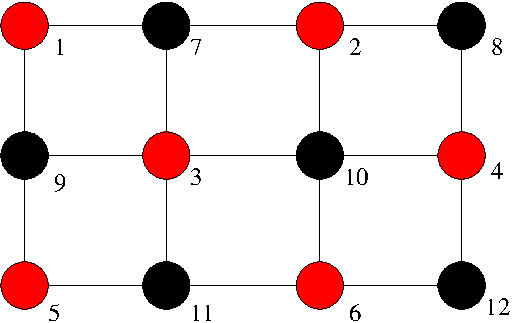
\includegraphics{ImplPic/RedBlack.pdf}}\par
Red Black
\end{minipage}
\begin{minipage}{3.2cm}
\centering
\resizebox{2.5cm}{!}{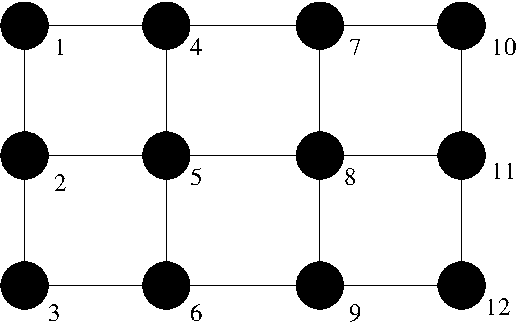
\includegraphics{ImplPic/LinearOrdering.pdf}}\par
Linear Ordering
\end{minipage}
\end{center}
\item So, the best ordering for the quality of the preconditioner is the one that is hardest to parallelize.
\item The ordering that we used is somewhat intermediate. It is like red-black globally, but over individual subdomains it is linear.
\end{itemize}
}


\frame{
\begin{center}
\begin{tabular*}{7cm}{c}
\\[-0.5cm]
{\Huge \textcolor{blue}{II. }\textcolor{red}{Solution}}\\[4mm]
{\Huge \textcolor{red}{for wave models}}
\end{tabular*}
\end{center}
}




\frame{
  \frametitle{Organizing the computation}
\begin{enumerate}
\item The penalty of parallelizing come in two ways:
\begin{enumerate}
\item The preconditioner quality that decreases.
\item The cost of waiting for data is $c$.
\end{enumerate}
\item If we have $N_{freq}$ frequencies and $N_{dir}$ directions then this makes $N_{tot}=N_{freq} \times N_{dir}$ independent linear systems to solve.
\item The strategy is then to split $N_{tot}$ into $b$ blocks $B_1$, \dots, $B_b$
\begin{enumerate}
\item After domains of color $1$ have finished block $B_1$ data is sent and block $B_2$ is solved.
\item So domains of color $2$ can start working before the ones of color $1$ are finished.
\end{enumerate}
\item So, by using say $b=5$ we can essentially remove the second cost.
\end{enumerate}
}


\frame{
  \frametitle{Further work}
\begin{enumerate}
\item The work done so far is for the SOR preconditioner.
\item We need to test the ILU0 preconditioner, it is harder to compute but the same strategy can be applied.
\item Another possibility is to integrate implicitly the advection in geographical, frequency and direction.\\
This requires an ordering of the $N_{node} \times N_{freq}\times N_{dir}$ matrix entries but by doing so we can diminish the splitting error.
\item And overall improve the speed.
\end{enumerate}
\begin{center}
\textcolor{blue}{THANK YOU}
\end{center}

}





\end{document}
